% answers.tex -- marking criteria and sample answers for questions.tex (Module 7 short answer).
% NESA marking-guideline style: a criteria table for each part, then a sample answer.
% Every number: checks/m7-short-answer/numbers.py
% Build: TEXINPUTS=.: xelatex answers.tex (twice)
\documentclass[12pt]{article}
\usepackage{quiz}
\hypersetup{pdftitle={Short Answer Questions - Module 7 - The Nature of Light - Marking guidelines}}
% links between the two PDF files are not possible, so question headings are plain text here
\renewcommand\hyperlink[2]{#2}
\newcommand\anstopic[1]{\par\Needspace{8\baselineskip}\vspace{4mm}%
  \begin{center}{\headfont\bfseries\fontsize{14}{18}\selectfont #1\par}\end{center}\vspace{2pt}}

\begin{document}
\quiztitle{Year 12 Physics}{Short Answer Questions - Module 7 - The Nature of Light:\\
  Marking Guidelines and Sample Answers}

Data used: $c = \qty{3.00e8}{m.s^{-1}}$, $h = \qty{6.626e-34}{J.s}$, $e = \qty{1.602e-19}{C}$,
$m_\mathrm{e} = \qty{9.109e-31}{kg}$, $m_\mathrm{p} = \qty{1.673e-27}{kg}$, $b = \qty{2.898e-3}{m.K}$.
In calculations, a correct answer from a correct method with an earlier error carried forward still
earns the later marks.

% =====================================================================
\anstopic{Topic 1 - Electromagnetic Spectrum}

% ---- Q1
\ansq
\anspart{a}
\begin{crit}
  \critrow{Outlines that the wave is made of oscillating electric and magnetic fields at right angles to
    each other and to the direction of travel, with a correctly labelled diagram}{2}
  \critrow{Gives ONE correct feature (for example, that the changing electric and magnetic fields produce
    each other), or a partly correct diagram}{1}
\end{crit}
\sample
According to Maxwell, a changing electric field produces a changing magnetic field, and a changing
magnetic field produces a changing electric field. The two fields keep producing each other, so they
travel through space as a wave, even through a vacuum. The electric and magnetic fields oscillate in
phase, at right angles to each other and at right angles to the direction of travel (a transverse wave).
\begin{center}
  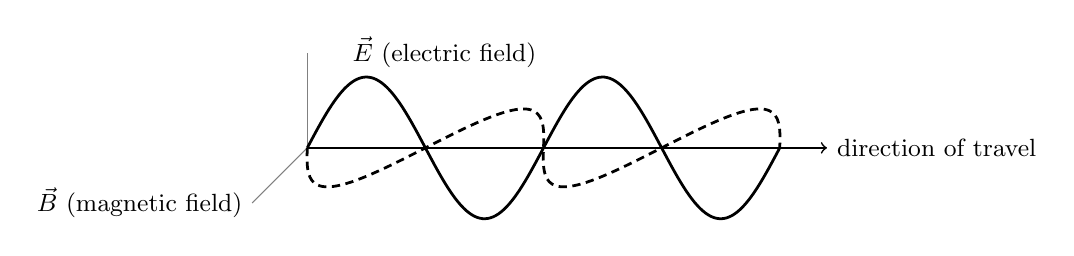
\begin{tikzpicture}
    \draw[->, line width=0.6pt] (0,0) -- (6.6,0) node[right, font=\small] {direction of travel};
    \draw[line width=0.4pt, black!50] (0,0) -- (0,1.2); \draw[line width=0.4pt, black!50] (0,0) -- (-0.7,-0.7);
    \draw[line width=1pt, domain=0:6, samples=90, smooth] plot (\x, {0.9*sin(\x*120)});
    \draw[line width=1pt, dash pattern=on 3pt off 2pt, domain=0:6, samples=90, smooth]
      plot ({\x - 0.55*0.9*sin(\x*120)}, {-0.55*0.9*sin(\x*120)});
    \node[above right, font=\small] at (0.45,0.9) {$\vec{E}$ (electric field)};
    \node[left, font=\small] at (-0.7,-0.7) {$\vec{B}$ (magnetic field)};
  \end{tikzpicture}
\end{center}
\anspart{b}
\begin{crit}
  \critrow{Correctly calculates the value AND explains its significance}{2}
  \critrow{Correctly calculates the value OR explains its significance}{1}
\end{crit}
\sample
$\dfrac{1}{\sqrt{\mu_0\varepsilon_0}} = \dfrac{1}{\sqrt{(4\pi\times10^{-7})(\num{8.854e-12})}}
= \qty{3.00e8}{m.s^{-1}}$, which is the measured speed of light. $\mu_0$ and $\varepsilon_0$ come from
experiments on magnetism and electricity, which have nothing to do with light. Maxwell concluded that light
is an electromagnetic wave. This joined electricity, magnetism and light into one theory, and predicted
other EM waves (such as radio waves, later produced by Hertz).

% ---- Q2
\ansq
\anspart{a}
\begin{crit}
  \critrow{Explains that, in the time the light takes to travel to the mirror and back, the wheel turns
    just far enough for the next tooth to move into the light's path}{2}
  \critrow{States that the returning light is blocked by a tooth, OR links the travel time of the light to
    the rotation of the wheel}{1}
\end{crit}
\sample
The light passes through a gap, travels \qty{15}{km} (there and back), and arrives back at the wheel a
short time later. At 20 revolutions per second, in this time the wheel turns by exactly the distance from
the middle of a gap to the middle of the next tooth. So the returning light hits a tooth and is blocked,
and the observer sees no light.
\anspart{b}
\begin{crit}
  \critrow{Correctly calculates the speed of light}{3}
  \critrow{Correctly calculates the time for the round trip, OR uses $c = \frac{2d}{t}$ with one
    error}{2}
  \critrow{Shows one relevant step (for example, the time for one revolution)}{1}
\end{crit}
\sample
One tooth plus one gap is $\frac{1}{500}$ of a turn, so from a gap to the next tooth is $\frac{1}{1000}$
of a turn. Time for this rotation:
\[ t = \frac{1}{1000 \times 20} = \qty{5.0e-5}{s}, \qquad
   c = \frac{2d}{t} = \frac{2 \times 7500}{\num{5.0e-5}} = \qty{3.0e8}{m.s^{-1}} \]

% ---- Q3
\ansq
\anspart{a}
\begin{crit}
  \critrow{Correctly calculates the temperature}{2}
  \critrow{Substitutes correctly into Wien's law}{1}
\end{crit}
\sample
$T = \dfrac{b}{\lambda_\mathrm{max}} = \dfrac{\num{2.898e-3}}{\num{414e-9}} = \qty{7.0e3}{K}$.
\anspart{b}
\begin{crit}
  \critrow{Relates the position of EACH star's curve (or peak) to the visible band, and explains the
    colours}{2}
  \critrow{Explains the colour of ONE star}{1}
\end{crit}
\sample
Star X peaks at \qty{414}{nm}, just at the violet end of the visible band. Across the visible band its
curve falls only gradually from the blue end to the red end, so it gives out a fairly even mix of all
colours (with a little more blue) and looks white. Star Y peaks at
$\frac{b}{T} = \frac{\num{2.898e-3}}{4500} = \qty{644}{nm}$, in the red part of the spectrum. Its curve rises
from the blue end to the red end of the visible band, so it emits much more red and orange light than
blue light: it looks orange-red.
\anspart{c}
\begin{crit}
  \critrow{Identifies star X and justifies using the graph (higher curve, larger area under the curve)}{1}
\end{crit}
\sample
Star X. Its curve is higher at every wavelength, so the area under its curve (the total energy emitted
per second from each square metre) is much larger.

% ---- Q4
\ansq
\anspart{a}
\begin{crit}
  \critrow{States that the star is moving away from Earth AND justifies it using the red shift of all
    the lines (Doppler effect)}{2}
  \critrow{States that the star is moving away, OR identifies a red shift}{1}
\end{crit}
\sample
All the star's lines are at longer wavelengths than the laboratory lines (a red shift), and the pattern of
lines is the same, so they are the same hydrogen lines. By the Doppler effect, light from a source moving
away is shifted to longer wavelengths. So the star is moving away from Earth.
\anspart{b}
\begin{crit}
  \critrow{Gives TWO valid reasons, each with a brief explanation}{2}
  \critrow{Gives ONE valid reason}{1}
\end{crit}
\sample
\begin{itemize}
  \item \textbf{Rotation:} one side of the star moves towards us and the other side moves away. Light from
        the two sides is blue-shifted and red-shifted by different amounts, so each line is spread out.
  \item \textbf{Density (pressure):} if the gas in the star's outer layers is dense, the atoms collide
        often, which widens the range of wavelengths each atom absorbs. (So the star is more likely to be a
        main-sequence star than a giant.)
\end{itemize}
(A higher temperature, which gives faster random motion of the atoms, is also accepted.)

% ---- Q5
\ansq
\anspart{a}
\begin{crit}
  \critrow{Identifies Elements 1 and 3 (and no others)}{1}
\end{crit}
\sample
Elements 1 and 3. (All their lines appear in the star. Element 2 has no matching lines. Element 4 has one
matching line, but its other line is missing, so it is not present.)
\anspart{b}
\begin{crit}
  \critrow{Explains how absorption lines form (continuous spectrum from the interior; cooler gas absorbs
    photons whose energy equals the gap between energy levels) AND why each element has a unique set of
    lines that matches its emission spectrum}{3}
  \critrow{Explains how absorption lines form, with limited link to identification}{2}
  \critrow{Gives one relevant point}{1}
\end{crit}
\sample
The hot, dense interior of the star emits a continuous spectrum. As this light passes through the cooler
gas in the outer layers, an atom can absorb a photon only if the photon's energy exactly equals the
difference between two of its energy levels ($hf = E_2 - E_1$). The absorbed energy is re-emitted in all
directions, so less light at these wavelengths reaches us, and dark lines appear. Each element has its own
set of energy levels, so it absorbs its own unique set of wavelengths. These are the same wavelengths as
the bright lines in its emission spectrum, so matching the star's dark lines with laboratory emission
spectra identifies the elements present.

% =====================================================================
\anstopic{Topic 2 - Light: Wave Model}

% ---- Q6
\ansq
\anspart{a}
\begin{crit}
  \critrow{Correctly calculates the fringe spacing}{2}
  \critrow{Substitutes correctly into $\Delta y = \frac{\lambda L}{d}$ (or $d\sin\theta = m\lambda$)}{1}
\end{crit}
\sample
$\Delta y = \dfrac{\lambda L}{d} = \dfrac{(\num{633e-9})(3.0)}{\num{0.25e-3}} = \qty{7.6e-3}{m} = \qty{7.6}{mm}$.
\anspart{b}
\begin{crit}
  \critrow{Explains bright fringes (path difference $m\lambda$, in phase, constructive) AND dark fringes
    (path difference $(m+\frac{1}{2})\lambda$, out of phase, destructive)}{2}
  \critrow{Explains bright OR dark fringes}{1}
\end{crit}
\sample
Light diffracts through each slit, and the two sets of waves overlap on the screen. Where the path
difference from the two slits is a whole number of wavelengths ($m\lambda$), the waves arrive in phase and
interfere constructively, giving a bright fringe. Where the path difference is $(m + \frac{1}{2})\lambda$,
they arrive out of phase and interfere destructively, giving a dark fringe.
\anspart{c}
\begin{crit}
  \critrow{Explains that interference is a wave property that the particle model could not explain}{1}
\end{crit}
\sample
Interference (light + light giving darkness) is a property of waves. Particles travelling in straight lines
from two slits would give just two bright bands, not a pattern of many evenly spaced bright and dark
fringes.

% ---- Q7
\ansq
\anspart{a}
\begin{crit}
  \critrow{Correctly calculates the angle}{2}
  \critrow{Correctly calculates the slit spacing $d$, OR substitutes into $d\sin\theta = m\lambda$}{1}
\end{crit}
\sample
$d = \dfrac{1}{\num{300e3}} = \qty{3.333e-6}{m}$. \quad
$\sin\theta = \dfrac{\lambda}{d} = \dfrac{\num{656e-9}}{\num{3.333e-6}} = 0.1968$, so $\theta = \ang{11.3}$
(accept \ang{11.3} to \ang{11.4}).
\anspart{b}
\begin{crit}
  \critrow{Correctly calculates the wavelength}{2}
  \critrow{Substitutes correctly into $d\sin\theta = m\lambda$}{1}
\end{crit}
\sample
$\lambda = d\sin\theta = (\num{3.333e-6})\sin 8.4^\circ = \qty{4.87e-7}{m}$ (\qty{487}{nm}, the blue-green
hydrogen line).
\anspart{c}
\begin{crit}
  \critrow{States the 5th order, with justification ($\sin\theta \le 1$)}{1}
\end{crit}
\sample
$\sin\theta = \frac{m\lambda}{d}$ cannot be more than 1, so $m \le \frac{d}{\lambda} = \frac{\num{3.33e-6}}{\num{656e-9}}
= 5.1$. The highest order is the 5th.

% ---- Q8
\ansq
\anspart{a}
\begin{crit}
  \critrow{\qty{30}{W.m^{-2}}}{1}
\end{crit}
\sample
A polarising filter halves the intensity of unpolarised light: $\frac{60}{2} = \qty{30}{W.m^{-2}}$.
\anspart{b}
\begin{crit}
  \critrow{Correctly calculates the intensity using Malus' law}{1}
\end{crit}
\sample
$I = I_\mathrm{max}\cos^2\theta = 30\cos^2 30^\circ = 30 \times 0.75 = \qty{22.5}{W.m^{-2}}$ (about
\qty{23}{W.m^{-2}}).
\anspart{c}
\begin{crit}
  \critrow{Explains that only transverse waves can be polarised, so light must be a transverse wave}{2}
  \critrow{States that light is a transverse wave, OR that polarisation supports the wave model}{1}
\end{crit}
\sample
Polarisation means restricting the oscillations of a wave to one plane. This is only possible for
transverse waves, whose oscillations are at right angles to the direction of travel. (Longitudinal waves,
such as sound, cannot be polarised.) Since light can be polarised, it must be a transverse wave. This
supports the wave model and Maxwell's prediction that light is a transverse EM wave. Malus' law also fits
the wave model: only the component $E\cos\theta$ of the electric field passes, and intensity is
proportional to the square of the amplitude.

% ---- Q9
\ansq
\begin{crit}
  \critrow{Compares the two models for several phenomena (for example refraction, including the speed in a
    denser medium, and diffraction or interference) AND assesses specific experimental evidence (for
    example Young and Foucault), reaching a clear judgement}{5}
  \critrow{Compares the models and refers to experimental evidence, with a judgement}{4}
  \critrow{Describes both models, with some comparison or some evidence}{3}
  \critrow{Describes features of one or both models}{2}
  \critrow{Gives some relevant information}{1}
\end{crit}
\sample
\begin{itemize}
  \item \textbf{Newton (particle model):} light is a stream of tiny particles. It explained straight-line
        travel, sharp shadows and reflection (like balls bouncing). It explained refraction by saying the
        particles are attracted by the denser medium, so it predicted that light travels \emph{faster} in
        water or glass. It could not easily explain diffraction or interference.
  \item \textbf{Huygens (wave model):} light is a wave, and every point on a wavefront acts as a source of
        new wavelets. It explained reflection and refraction, predicting that light travels \emph{slower}
        in a denser medium. Huygens' principle could also explain diffraction (light bending around edges).
  \item \textbf{Similarities:} both models explained reflection and refraction, and both gave the law of
        refraction (Snell's law).
  \item \textbf{Evidence:} because of Newton's reputation, the particle model was accepted for about 100
        years. Then Young's double-slit experiment (1801) showed interference, which only waves could
        explain. Foucault (1850) measured the speed of light in water and found it was \emph{lower} than in
        air, as the wave model predicted and against Newton's model.
  \item \textbf{Judgement:} the experimental evidence clearly decided in favour of Huygens' wave model. This
        shows that a model is accepted because its predictions agree with experiments, not because of who
        proposed it. (Later, the photoelectric effect showed that light also has particle properties.)
\end{itemize}

% ---- Q10
\ansq
\begin{crit}
  \critrow{Describes a valid method with the measurements made, explains how $\lambda$ is calculated, AND
    gives a valid way to improve accuracy}{4}
  \critrow{Describes a valid method with most of these features}{3}
  \critrow{Describes some relevant steps or the calculation}{2}
  \critrow{Gives one relevant point}{1}
\end{crit}
\sample
\begin{itemize}
  \item Shine the laser at right angles through a diffraction grating of known lines per mm (for example
        300 lines/mm, so $d = \frac{1}{\num{300e3}}$ m) onto a screen or wall about \qty{1}{m} away.
  \item Measure the distance $L$ from the grating to the screen with a metre ruler.
  \item Mark the central maximum and the first-order maxima on each side. Measure the distance between
        the two first-order maxima, and halve it to get $x$.
  \item Calculate $\theta = \tan^{-1}\!\left(\frac{x}{L}\right)$, then $\lambda = \frac{d\sin\theta}{m}$ with
        $m = 1$.
  \item \textbf{Improving accuracy:} measure between the maxima on \emph{both} sides and halve (this
        removes the error from not knowing the exact centre); use a larger $L$ so the distances are larger
        and the percentage uncertainty is smaller; repeat for several values of $L$ (or use higher orders)
        and average. Work in a darkened room so the maxima are easy to locate.
  \item Safety: never look into the laser beam or its reflections.
\end{itemize}

% =====================================================================
\anstopic{Topic 3 - Light: Quantum Model}

% ---- Q11
\ansq
\anspart{a}
\begin{crit}
  \critrow{Correctly calculates the wavelength}{1}
\end{crit}
\sample
$\lambda_\mathrm{max} = \dfrac{b}{T} = \dfrac{\num{2.898e-3}}{5800} = \qty{5.0e-7}{m}$ (\qty{500}{nm}).
\anspart{b}
\begin{crit}
  \critrow{Describes the classical prediction (intensity increasing without limit at short wavelengths)
    and the observed curves (a peak, then falling to zero), AND explains Planck's quantisation and how it
    reduces the short-wavelength emission}{3}
  \critrow{Describes the problem AND states Planck's hypothesis}{2}
  \critrow{Gives one relevant point}{1}
\end{crit}
\sample
Classical physics treated the radiation as waves whose energy could take any value, with energy shared
equally among all possible waves. There are more and more possible waves at shorter wavelengths, so it
predicted that the intensity would increase without limit as the wavelength gets shorter: the
``ultraviolet catastrophe''. The observed curves instead rise to a peak and then fall to zero at short
wavelengths. Planck (1900) assumed that the energy of the oscillators in a black body is quantised: it can
only be a whole-number multiple of $hf$. High-frequency (short-wavelength) oscillations need a large
amount of energy for even one quantum, so they are rarely excited, and very little short-wavelength
radiation is emitted. His formula matched the observed curves at all wavelengths, and this was the start
of quantum theory.

% ---- Q12
\ansq
\anspart{a}
\begin{crit}
  \critrow{Correctly calculates the photon energy in eV}{1}
\end{crit}
\sample
$E = \dfrac{hc}{\lambda} = \dfrac{(\num{6.626e-34})(\num{3.00e8})}{\num{400e-9}} = \qty{4.97e-19}{J}$;
\quad $\dfrac{\num{4.97e-19}}{\num{1.602e-19}} = \qty{3.10}{eV}$.
\anspart{b}
\begin{crit}
  \critrow{Correctly calculates $K_\mathrm{max}$ in joules}{1}
\end{crit}
\sample
$K_\mathrm{max} = hf - \phi = 3.10 - 2.3 = \qty{0.80}{eV} = 0.80 \times \num{1.602e-19} = \qty{1.28e-19}{J}$.
\anspart{c}
\begin{crit}
  \critrow{Correctly calculates the maximum speed}{2}
  \critrow{Uses $K = \frac{1}{2}mv^2$ with the mass of the electron}{1}
\end{crit}
\sample
$v = \sqrt{\dfrac{2K}{m}} = \sqrt{\dfrac{2(\num{1.28e-19})}{\num{9.109e-31}}} = \qty{5.3e5}{m.s^{-1}}$.
\anspart{d}
\begin{crit}
  \critrow{\qty{0.80}{V}}{1}
\end{crit}
\sample
$eV_0 = K_\mathrm{max}$, so $V_0 = \dfrac{\num{1.28e-19}}{\num{1.602e-19}} = \qty{0.80}{V}$.

% ---- Q13
\ansq
\anspart{a}
\begin{crit}
  \critrow{Correctly calculates the gradient from two points on the line, and identifies it as $h$}{2}
  \critrow{Identifies the gradient as $h$, OR calculates the gradient with a minor error}{1}
\end{crit}
\sample
$K_\mathrm{max} = hf - \phi$, so the gradient is $h$. Using $(\num{5.5e14}, 0)$ and
$(\num{10.0e14}, \num{3.0e-19})$:
\[ h = \frac{\num{3.0e-19} - 0}{\num{10.0e14} - \num{5.5e14}} = \qty{6.7e-34}{J.s} \]
\anspart{b}
\begin{crit}
  \critrow{Reads the threshold frequency AND correctly calculates the work function in eV}{2}
  \critrow{Reads the threshold frequency, OR calculates $\phi$ in joules only}{1}
\end{crit}
\sample
The line cuts the $f$ axis at the threshold frequency $f_0 = \qty{5.5e14}{Hz}$.
$\phi = hf_0 = (\num{6.7e-34})(\num{5.5e14}) = \qty{3.7e-19}{J}$;
$\dfrac{\num{3.7e-19}}{\num{1.602e-19}} = \qty{2.3}{eV}$.
(Using $h = \qty{6.626e-34}{J.s}$ gives the same answer to two significant figures.)
\anspart{c}
\begin{crit}
  \critrow{A parallel line (same gradient) with a larger threshold frequency (shifted to the right)}{1}
\end{crit}
\sample
The line would be parallel to this one (the gradient is still $h$), but shifted to the right: it would cut
the $f$ axis at a higher threshold frequency.

% ---- Q14
\ansq
\begin{crit}
  \critrow{For TWO observations, explains why the wave model fails AND how Einstein's photon model
    accounts for it}{4}
  \critrow{Does this fully for one observation and partly for the other}{3}
  \critrow{Explains one observation, OR describes Einstein's model with some link to observations}{2}
  \critrow{Gives one relevant point}{1}
\end{crit}
\sample
Einstein proposed that light is made of photons, each with energy $E = hf$, and that each photon gives all
its energy to one electron. An electron escapes if $hf > \phi$, with $K_\mathrm{max} = hf - \phi$.
\begin{itemize}
  \item \textbf{Threshold frequency:} no electrons are emitted below a certain frequency, however bright
        the light. In the wave model, the energy depends on intensity, so bright enough light of any
        frequency should release electrons. In Einstein's model, if $hf < \phi$ no single photon has enough
        energy, and more photons do not help, because an electron absorbs only one photon.
  \item \textbf{$K_\mathrm{max}$ depends on frequency, not intensity:} the wave model predicted that brighter
        light would give the electrons more energy. In Einstein's model, brighter light means more photons,
        so more electrons, but each photon still has energy $hf$, so $K_\mathrm{max} = hf - \phi$ is
        unchanged. A higher frequency gives each photon more energy, so $K_\mathrm{max}$ increases.
  \item (Also accepted) \textbf{No time delay:} the wave model predicted that dim light would need time to
        build up enough energy. In Einstein's model, one photon delivers its energy at once.
\end{itemize}

% ---- Q15
\ansq
\anspart{a}
\begin{crit}
  \critrow{Correctly calculates the photon energy}{1}
\end{crit}
\sample
$E = \dfrac{hc}{\lambda} = \dfrac{(\num{6.626e-34})(\num{3.00e8})}{\num{532e-9}} = \qty{3.74e-19}{J}$.
\anspart{b}
\begin{crit}
  \critrow{Correctly calculates the number of photons per second}{1}
\end{crit}
\sample
$N = \dfrac{P}{E} = \dfrac{\num{2.0e-3}}{\num{3.74e-19}} = \num{5.4e15}$ photons per second.
\anspart{c}
\begin{crit}
  \critrow{Calculates both photon energies and compares them with the work function, explaining that one
    photon releases one electron, so intensity (power) does not matter}{2}
  \critrow{Calculates the infrared photon energy, OR explains in terms of photon energy without
    calculation}{1}
\end{crit}
\sample
Green photon: $\qty{3.74e-19}{J} = \qty{2.33}{eV}$, which is more than \qty{2.0}{eV}, so each photon can
release an electron. Infrared photon:
$E = \dfrac{(\num{6.626e-34})(\num{3.00e8})}{\num{1200e-9}} = \qty{1.66e-19}{J} = \qty{1.03}{eV}$, which is
less than \qty{2.0}{eV}. Each electron absorbs only one photon, so no infrared photon can release an
electron. The lamp's much greater power only means more photons per second, not more energy per photon.

% =====================================================================
\anstopic{Topic 4 - Light and Special Relativity}

% ---- Q16
\ansq
\begin{crit}
  \critrow{Explains that the light travels a longer (diagonal) path in the frame where the clock moves,
    that by the second postulate it travels at the same speed $c$ in both frames, and therefore the time
    for each tick is longer (time dilation)}{4}
  \critrow{Explains most of these points}{3}
  \critrow{Identifies the longer path OR the constant speed of light, with a link to time}{2}
  \critrow{Gives one relevant point}{1}
\end{crit}
\sample
For the observer moving with the clock, the light goes straight up and down, a distance $2L$ for one tick,
so $t_0 = \frac{2L}{c}$. This is the proper time, because the tick starts and ends at the same place in
this frame. For the observer who sees the clock moving, the mirrors move sideways while the light travels,
so the light follows a longer, diagonal path. By Einstein's second postulate, the speed of light is $c$ for
both observers (it does not add to the speed of the clock, as Galilean relativity would suggest). A longer
distance at the same speed takes a longer time, so this observer measures a longer time for each tick: the
moving clock runs slow. Using Pythagoras' theorem on the diagonal path,
$\left(\frac{ct}{2}\right)^2 = L^2 + \left(\frac{vt}{2}\right)^2$, which gives
$t = \dfrac{t_0}{\sqrt{1 - v^2/c^2}}$. By the first postulate, both observers' measurements are equally
valid; neither is ``really'' at rest.

% ---- Q17
\ansq
\anspart{a}
\begin{crit}
  \critrow{Correctly calculates the distance}{1}
\end{crit}
\sample
$d = vt = (0.998 \times \num{3.00e8})(\num{2.2e-6}) = \qty{6.6e2}{m}$ (about \qty{0.66}{km}).
\anspart{b}
\begin{crit}
  \critrow{Correctly calculates the dilated lifetime AND the distance}{2}
  \critrow{Correctly calculates $\gamma$ or the dilated lifetime}{1}
\end{crit}
\sample
$\gamma = \dfrac{1}{\sqrt{1 - 0.998^2}} = 15.8$. \quad $t = \gamma t_0 = 15.8 \times \qty{2.2}{\micro s}
= \qty{35}{\micro s}$. \quad $d = vt = (0.998 \times \num{3.00e8})(\num{34.8e-6}) = \qty{1.04e4}{m}$
(about \qty{10.4}{km}).
\anspart{c}
\begin{crit}
  \critrow{Correctly calculates the contracted thickness}{1}
\end{crit}
\sample
$L = \dfrac{L_0}{\gamma} = \dfrac{10}{15.8} = \qty{0.63}{km}$.
\anspart{d}
\begin{crit}
  \critrow{Explains that without relativity few muons would reach the ground, but time dilation (or length
    contraction) allows them to}{1}
\end{crit}
\sample
Without relativity, a typical muon would travel only about \qty{0.66}{km} before decaying, so very few
would reach the ground from \qty{10}{km}. Many are detected, as special relativity predicts: in Earth's
frame their lifetime is dilated to \qty{35}{\micro s}, and in the muons' frame the atmosphere is only
\qty{0.63}{km} thick. Both frames agree that the muons reach the ground.

% ---- Q18
\ansq
\anspart{a}
\begin{crit}
  \critrow{\qty{5.25}{years}}{1}
\end{crit}
\sample
$t = \dfrac{d}{v} = \dfrac{\qty{4.2}{ly}}{0.80c} = \qty{5.25}{years}$ (a light-year is the distance light
travels in one year).
\anspart{b}
\begin{crit}
  \critrow{Correctly calculates the astronauts' time, using $t_0 = \frac{t}{\gamma}$}{2}
  \critrow{Correctly calculates $\gamma$, OR identifies the astronauts' time as the proper time}{1}
\end{crit}
\sample
$\gamma = \dfrac{1}{\sqrt{1 - 0.80^2}} = \dfrac{1}{0.60} = 1.67$. The astronauts measure the proper time,
because the departure and arrival happen at the same place in their frame (the ship):
$t_0 = \dfrac{t}{\gamma} = 5.25 \times 0.60 = \qty{3.15}{years}$.
\anspart{c}
\begin{crit}
  \critrow{Correctly calculates the contracted distance}{1}
\end{crit}
\sample
$L = \dfrac{L_0}{\gamma} = 4.2 \times 0.60 = \qty{2.52}{ly}$.
\anspart{d}
\begin{crit}
  \critrow{Shows that the contracted distance divided by $0.80c$ gives the astronauts' time}{1}
\end{crit}
\sample
In the astronauts' frame, the star comes towards them at $0.80c$ and has \qty{2.52}{ly} to cover:
$t = \dfrac{2.52}{0.80} = \qty{3.15}{years}$, the same as in (b).

% ---- Q19
\ansq
\anspart{a}
\begin{crit}
  \critrow{Correctly calculates the relativistic momentum}{2}
  \critrow{Correctly calculates $\gamma$, OR calculates the classical momentum}{1}
\end{crit}
\sample
$\gamma = \dfrac{1}{\sqrt{1 - 0.95^2}} = 3.20$. \quad
$p = \gamma m v = 3.20 \times (\num{1.673e-27}) \times (0.95 \times \num{3.00e8}) = \qty{1.5e-18}{kg.m.s^{-1}}$.
\anspart{b}
\begin{crit}
  \critrow{Correctly calculates the rest energy}{1}
\end{crit}
\sample
$E_0 = mc^2 = (\num{1.673e-27})(\num{3.00e8})^2 = \qty{1.5e-10}{J}$.
\anspart{c}
\begin{crit}
  \critrow{Explains that as $v \to c$, $\gamma$ (and so the energy and momentum) increases without limit,
    so reaching $c$ would need infinite energy}{2}
  \critrow{States that infinite energy would be needed, OR that $\gamma$ becomes infinite at $c$}{1}
\end{crit}
\sample
The proton's total energy is $\gamma mc^2$ and its momentum is $\gamma mv$. As $v$ gets closer to $c$,
$\gamma = \frac{1}{\sqrt{1 - v^2/c^2}}$ increases without limit. Reaching $c$ would need infinite energy,
which is impossible. Extra energy increases $\gamma$ (and the momentum), but produces smaller and smaller
increases in speed, so the speed always stays below $c$.

% ---- Q20
\ansq
\begin{crit}
  \critrow{Explains the aether idea, the expected result and the null result of the Michelson--Morley
    experiment, AND how Einstein's postulates removed the need for the aether and made $c$ the same for all
    observers}{4}
  \critrow{Explains most of these points}{3}
  \critrow{Describes the experiment or the postulates, with a link to the aether}{2}
  \critrow{Gives one relevant point}{1}
\end{crit}
\sample
In the 19th century, light was thought to be a wave that needed a medium, the ``aether'', which filled
space and was at absolute rest. As Earth moves through the aether, the speed of light measured on Earth
should depend on its direction (an ``aether wind''). In 1887, Michelson and Morley used an interferometer
to compare light travelling along two perpendicular arms. Rotating the apparatus should have shifted the
interference fringes, but no shift was found (a null result): there was no evidence of the aether. In 1905
Einstein postulated that (1) the laws of physics are the same in all inertial frames of reference, and
(2) the speed of light in a vacuum is the same for all observers. This made the aether unnecessary: light
needs no medium, there is no absolute frame of rest, and $c$ is constant whatever the motion of the source
or observer. Instead, time and length depend on the observer (time dilation and length contraction).

\end{document}
